\documentclass[a4paper,twoside,12pt]{article}
\usepackage{../z/zed-cm}
\usepackage{graphicx}
\usepackage[nottoc,numbib]{tocbibind}
\markboth{Draft}{Version 0.1}
\pagestyle{myheadings}
\begin{document}
\parskip 2 pt
\parindent 10 pt

\def\Slash{\slash\hspace{0pt}}

\title{A Container description}

\author{
Glyn Normington\and
Steve Powell
}

\maketitle
% The following three commands ensure the title page is without a page number but page numbering starts here.
% Page numbers appear on subsequent pages, and are roman until the main body, which starts again at arabic 1.
\thispagestyle{empty}
\pagenumbering{roman}
\setcounter{page}{1}

%=============================================================================

This document attempts to describe containers \cite{containers} in a precise fashion.

% Alt-Cmd-M -- \emph{}
% Alt-Cmd-Z -- \zed{}
% Alt-Cmd-X -- \axdef{}
% Alt-Cmd-S -- \schema{}
% Alt-Shift-Cmd-T -- \texttt{}

% Type checking hacks
\newcommand{\true}{true}
\newcommand{\false}{false}
\renewcommand{\emptyset}{\varnothing}
%=============================================================================

\clearpage
\tableofcontents

\cleardoublepage
\pagenumbering{arabic}
\setcounter{page}{1}

%=============================================================================
\section{Introduction}

This is a document that records the deliberations of Glyn and Steve as they come to grips with ``what containers really
are''\footnote{``What \emph{are} containers?'' \emph{Jerzy Czaykowski} (adapted)}.

%=============================================================================
\section{Overview of this document}

This document is a rag-bag of concepts and ideas (at the moment). The intention is to find the right decomposition of ideas to simply describe the state, and state transitions, of \emph{Containers} and the \emph{Jobs} that they \emph{Run}.


%=============================================================================
\section{Initial whiteboard stuff}

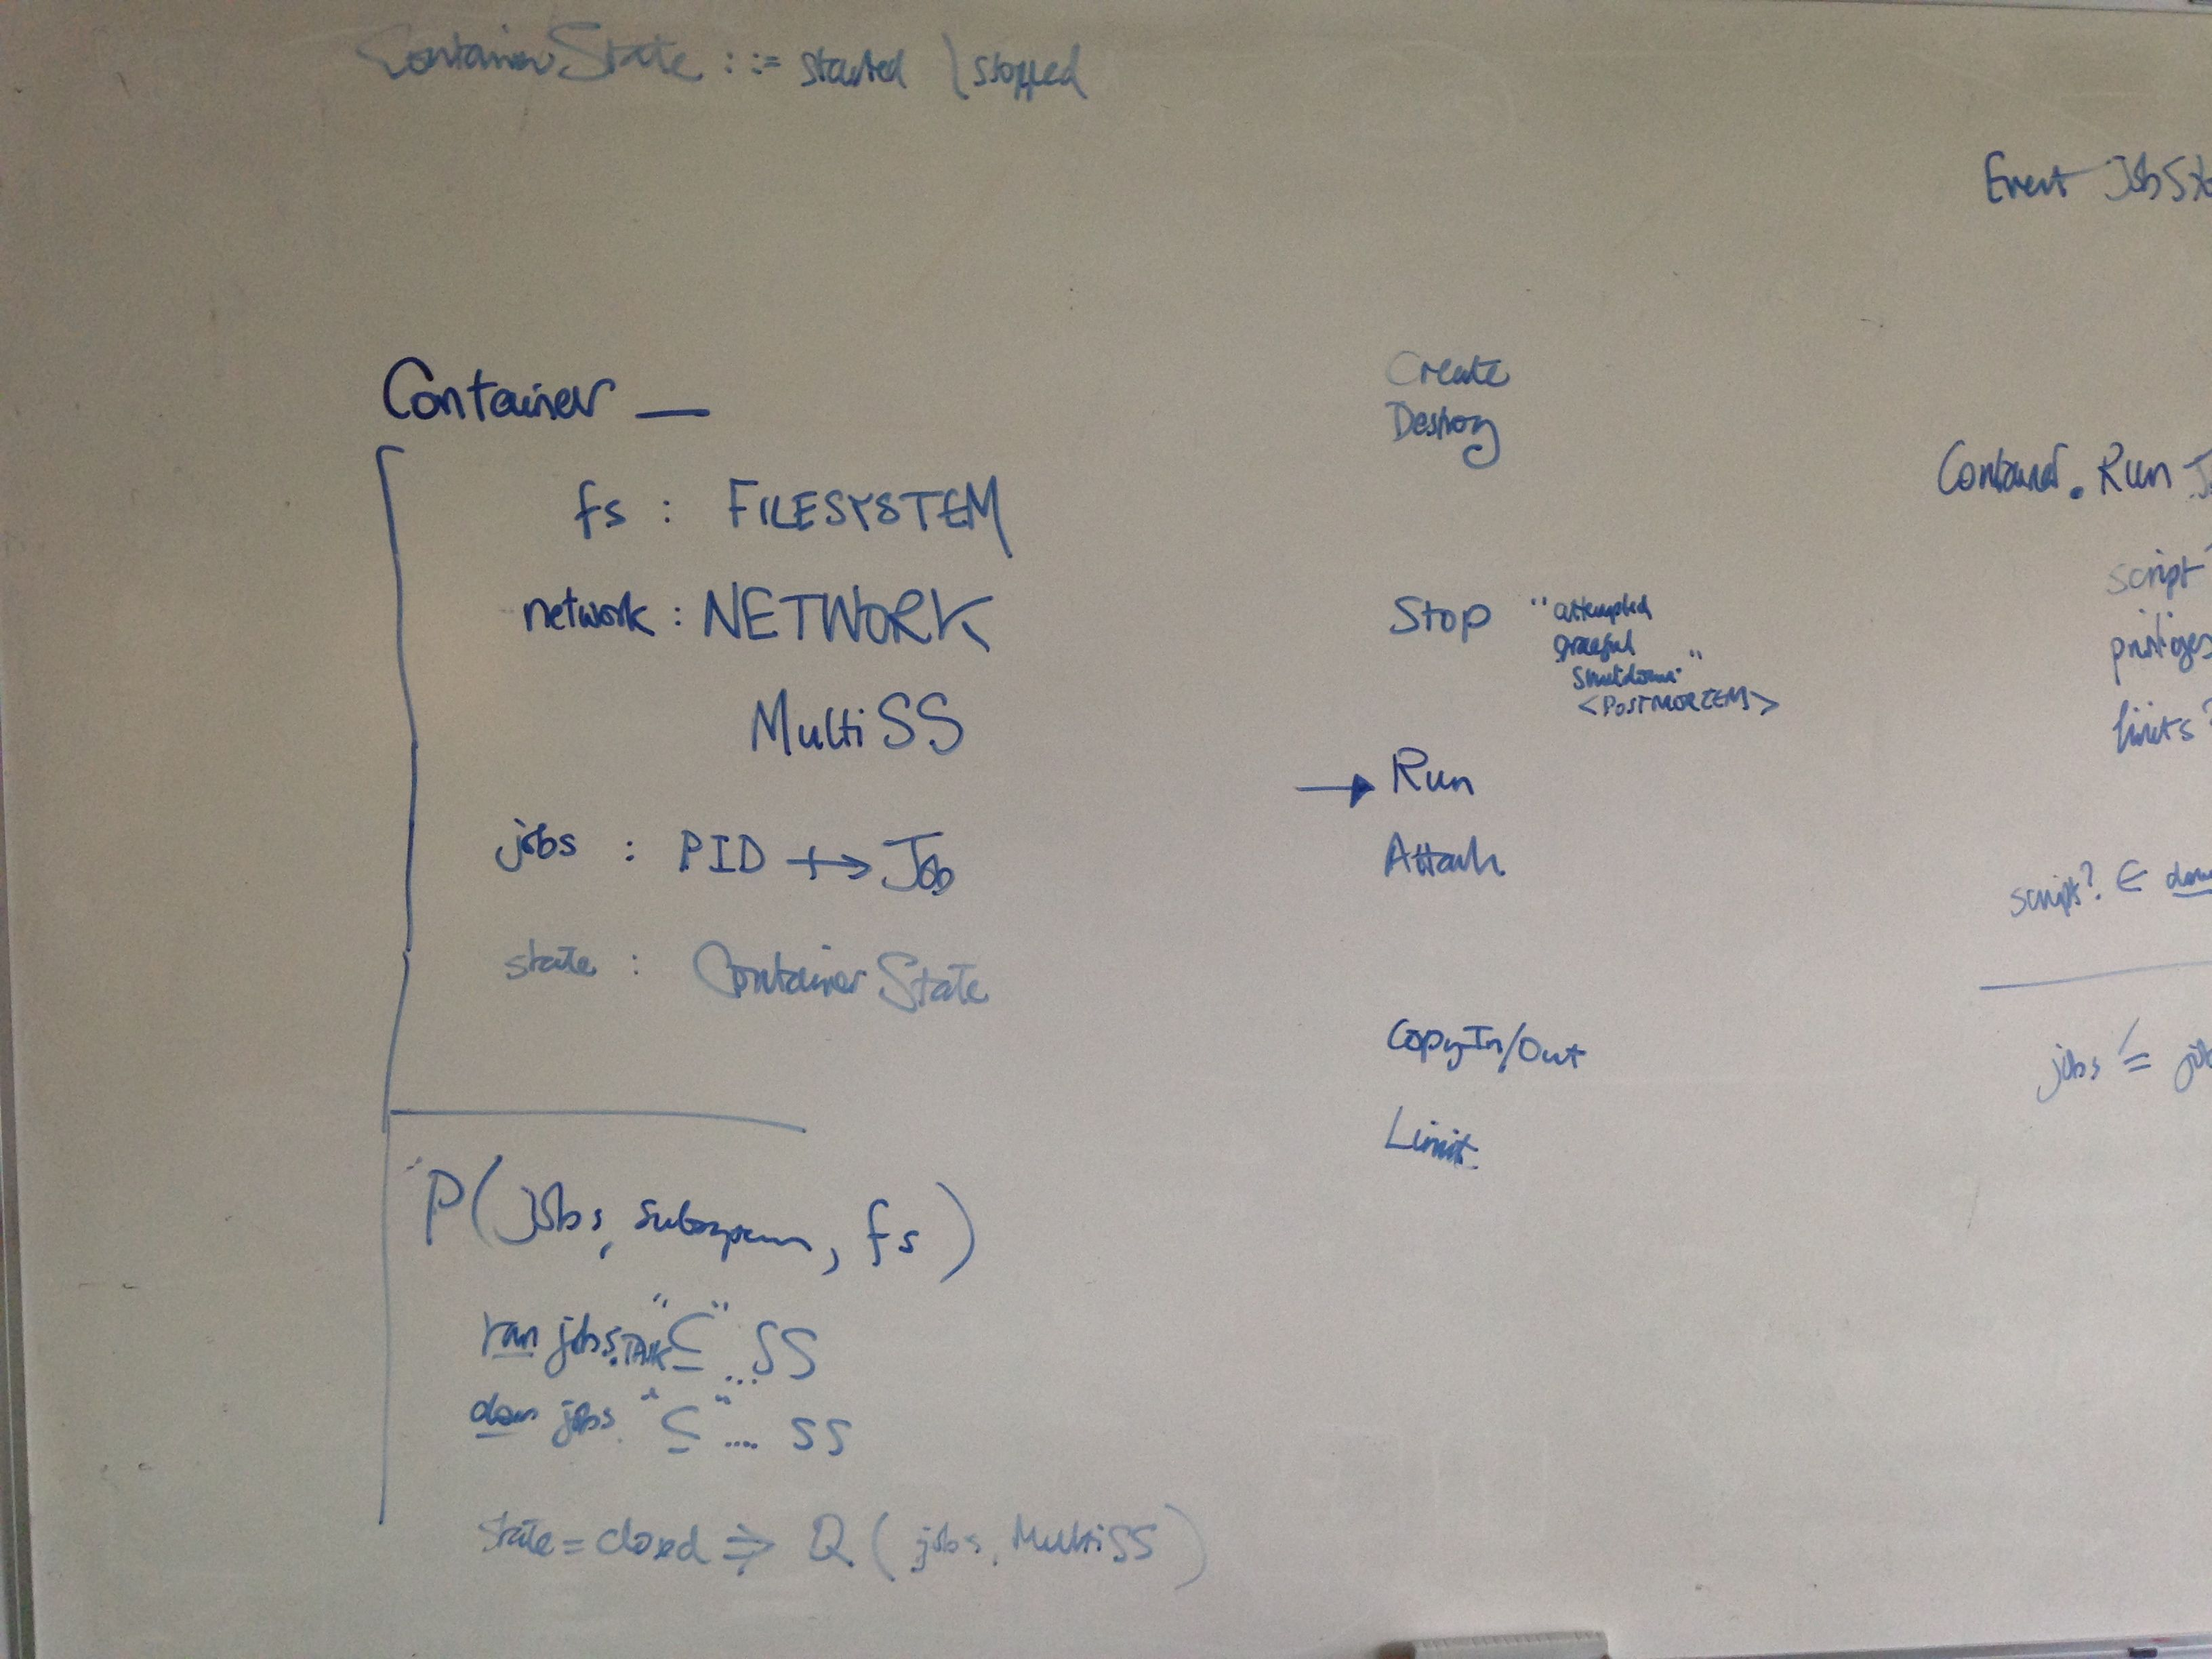
\includegraphics[width=\textwidth]{pics/IMG_0685.jpg}

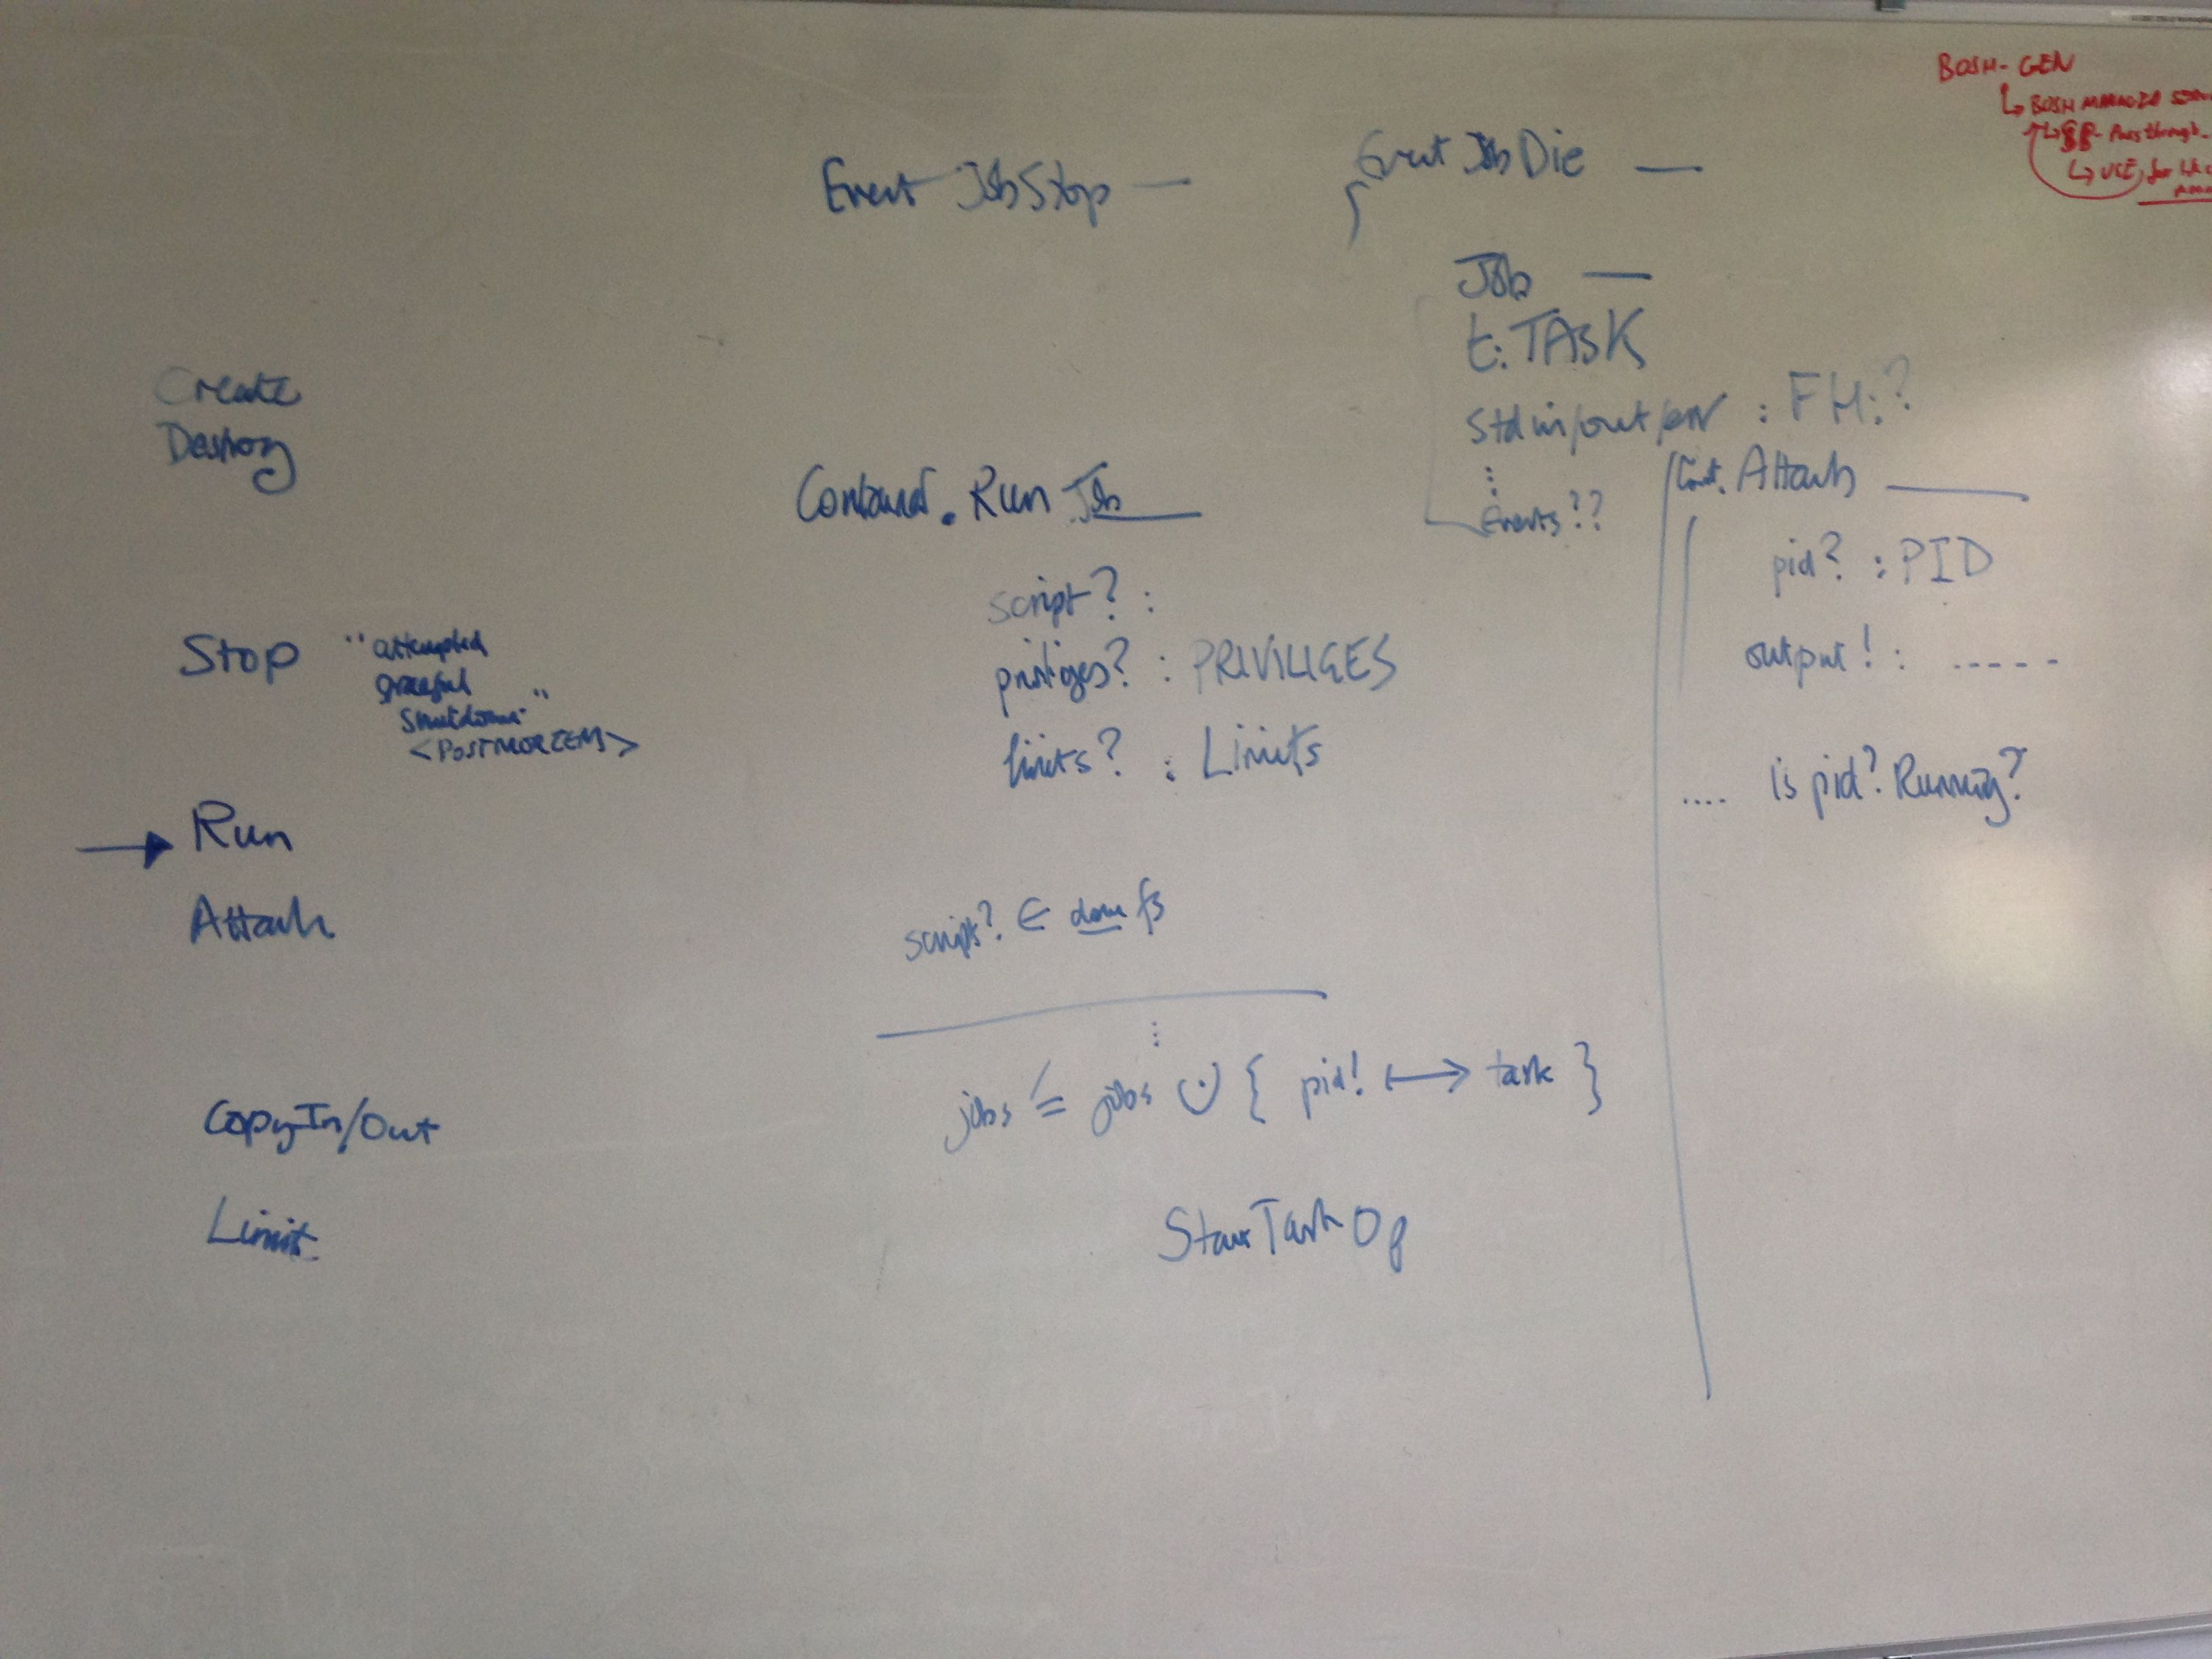
\includegraphics[width=\textwidth]{pics/IMG_0686.jpg}

%=============================================================================
%   B I B L I O G R A P H Y
%=============================================================================
\newpage
\begin{flushleft}
\begin{thebibliography}{99}
\label{sec:references}
% `99' is a picture of the generated numeric references -- they are two digits in this bibliography
% If we had a hundred or more we would have used 999, or whatever.

%%  Example bibliography entry:
%\bibitem{knuth76}                                                        % citation callout, e.g.: \cite{knuth76}
%  Donald E. Knuth,                                                        % author
%  \emph{The computer as Master Mind}.                    % title
%  J. Recreational Mathematics, Vol.~9(1), 1976-1977. % publisher, or journal, volume and date

\bibitem{warden}
  Various authors,
  \emph{Warden github repository},
  \texttt{https://github.com/cloudfoundry/warden}.

\bibitem{garden}
  Various authors,
  \emph{Garden github repository},
  \texttt{https://github.com/pivotal-cf-experimental/garden}.

% API abstracting the cgroup filesystem
% See http://manpages.ubuntu.com/manpages/lucid/man5/cgconfig.conf.5.html for configuration containing useful insights
\bibitem{libcgroup}
  Various authors
  \emph{libcgroup},
  {\small \texttt{http://libcg.sourceforge.net/html/index.html}}.

\bibitem{linuxgroups}
  Paul Menage, Paul Jackson and Christoph Lameter,
  \emph{CGROUPS},
  {\small \texttt{https://www.kernel.org/doc/Documentation/cgroups/cgroups.txt}}, 2004-2006.

\bibitem{linuxkernel}
  Linus Torvalds, \emph{et al},
  \emph{Linux kernel source tree},
  {\small \texttt{https://github.com/torvalds/linux}}.

\bibitem{memory}
  Various authors,
  \emph{Memory Resource Controller},
  {\small \texttt{https://www.kernel.org/doc/Documentation/cgroups/memory.txt}}.

\bibitem{noop}
  Kamezawa Hiroyuki, \emph{et al},
  \emph{NOOP cgroup subsystem},
  {\small \texttt{http://thread.gmane.org/gmane.linux.kernel/777763}}.

\bibitem{rharticle}
  Martin Prpi\u{c}, R\"udiger Landmann, and Douglas Silas,
  \emph{Red Hat Enterprise Linux 6.5 GA: Resource Management Guide},
  {\small \texttt{https://access.redhat.com/site/documentation/en-US\slash{}Red\_Hat\_Enterprise\_Linux/6/pdf/Resource\_Management\_Guide\slash{}Red\_Hat\_Enterprise\_Linux-6-Resource\_Management\_Guide-en-US.pdf}}.

\bibitem{7sins}
  Bertrand Meyer,
  \emph{On Formalism In Specifications},
  IEEE Software, Vol.~2(1), 1985.
\end{thebibliography}
\end{flushleft}
\end{document}
